\documentclass[12pt]{article}
\usepackage[english]{babel}
\usepackage{natbib}
\usepackage{url}
\usepackage[utf8x]{inputenc}
\usepackage{amsmath}
\usepackage{graphicx}
\graphicspath{{images/}}
\usepackage{parskip}
\usepackage{fancyhdr}
\usepackage{vmargin}
\usepackage{xcolor}
\usepackage{siunitx}
\usepackage{physics}


\setmarginsrb{3 cm}{2 cm}{3 cm}{2 cm}{1 cm}{1.5 cm}{1 cm}{1.5 cm}

\title{Lab 10}													% Title
\author{G 03}														% Author
\date{11 june 2019}														% Date

\makeatletter
\let\thetitle\@title
\let\theauthor\@author
\let\thedate\@date
\makeatother

\pagestyle{fancy}
\fancyhf{}
\rhead{\theauthor}
\lhead{\thetitle}
\cfoot{\thepage}
\newcommand{\mis}[3]{(#1 \pm #2) \ #3}
\newcommand{\misp}[3]{(#1 \#3 \pm #2}
\begin{document}

%%%%%%%%%%%%%%%%%%%%%%%%%%%%%%%%%%%%%%%%%%%%%%%%%%%%%%%%%%%%%%%%%%%%%%%%%%%%%%%%%%%%%%%%%

\begin{titlepage}
	\centering
    \vspace*{0.5 cm}
    
\includegraphics[scale = 0.75]{polito.jpg}\\[1.0 cm]				% University Logo
    \textsc{\LARGE Politecnico di Torino}\\[2.0 cm]						% University Name
	\textsc{\Large Digital systems electronics\\ A.A. 2018/2019}\\[0.5 cm]		% Course Code
	\textsc{\Large Prof. G. Masera}\\[0.5 cm]		% Nome del Professore
	\rule{\linewidth}{0.2 mm} \\[0.4 cm]
	{ \huge \bfseries \thetitle \\ \small \thedate}\\
	\rule{\linewidth}{0.2 mm} \\[1.5 cm]
	
	\begin{minipage}{0.4\textwidth}
		\begin{flushleft} \large
			Berchialla Luca\\												%Cognomi e nomi
			Laurasi Gjergji
			\\
			
			Mattei Andrea\\
            Lombardo Domenico Maria\\
            Wylezek Karolina
            
			\end{flushleft}
			\end{minipage}~
			\begin{minipage}{0.4\textwidth}
            
			\begin{flushright} \large
			236032\\													%Matricole
			238259\\
            233755\\
            233959\\
            267219\\
            
		\end{flushright}
        
	\end{minipage}\\[2 cm]
	
\end{titlepage}

%%%%%%%%%%%%%%%%%%%%%%%%%%%%%%%%%%%%%%%%%%%%%%%%%%%%%%%%%%%%%%%%%%%%%%%%%%%%%%%%%%%%%%%%%
\newpage

\section*{1 Measuring the frequency and the duty cycle of a squarewave }

The first task of the laboratory consists in measuring the frequency of a squarewave using the input capture function of timer 3 (TIM3). The input squarewave is received on the pin PA6.
The only code present in "main.c" file (aside from the one generated by CubeMX) is the one used for enabling timer in input capture mode and the relative interrupt.
In the TIM3 interrupt function, after checking if the interrupt has been called by the given input capture, the value of the time stamp of the rising or falling edge is saved in a variable. After the second rising edge the period is calculated as the difference between the 2 rising edge stamps by the prescaler and divided by the clock frequency, similarly the duty cycle is measured by capturing the falling edge event. In this way, both positive and negative semi period can be independently measured.

The prescaler has been set in order to have a 42kHz frequency (prescaler:1999), therefore in case of 100Hz waves the timer cannot reset multiple time.

If we put the break-point where we haven't already acquired all the count0, count1, count2 we can't get the right value because even tough the execution of the code is stopped, the counter continue counting.

The maximum detectable frequency is equal to the counter's clock frequency because we have at least to count to 1, so to increase it we can lower the prescaler value. The minimum detectable frequency in our code is equal to the counter's clock times $2^{16}$ which is the value of the ARR register. Actually we can further increase the maximum detectable period if we keep track of the ARR flag. \\
To increase the resolution of the measurement of a single period we have to increase the clock frequency by lowering the prescaler value.


\newpage
\section*{2.1 Generating a square wave}
The code for this task is very similar to the one of the previous part. A square wave with frequency 100Hz and duty cycle ranging between 25\% and 75\% has been generated using the PWM function of the timer 3 on pin PA6. In order to have the desired frequency the prescaler was set to 10 and the auto-reload was to set to 42. The changing DC is set up by reading the frequency of a sample input square wave.

\begin{figure}[h!]
	\centering
	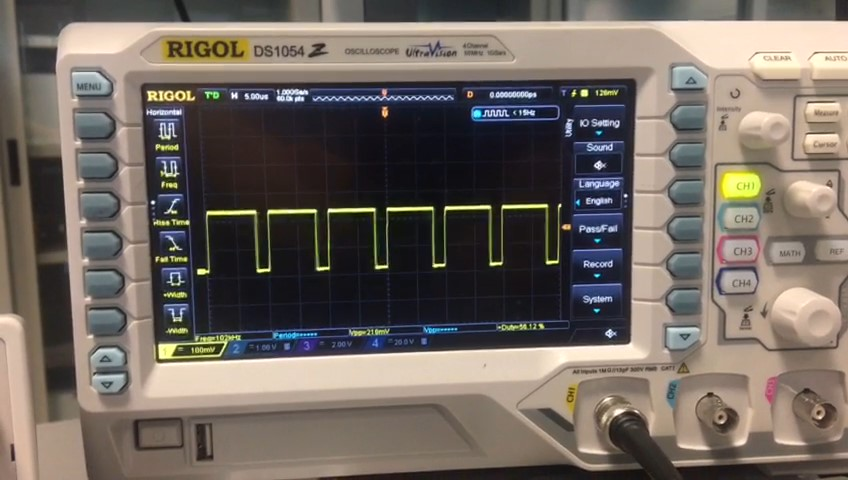
\includegraphics[scale = 0.4]{immagini/Whs.jpg}
	\caption{DC=75\%}
\end{figure}

\begin{figure}[h!]
\centering
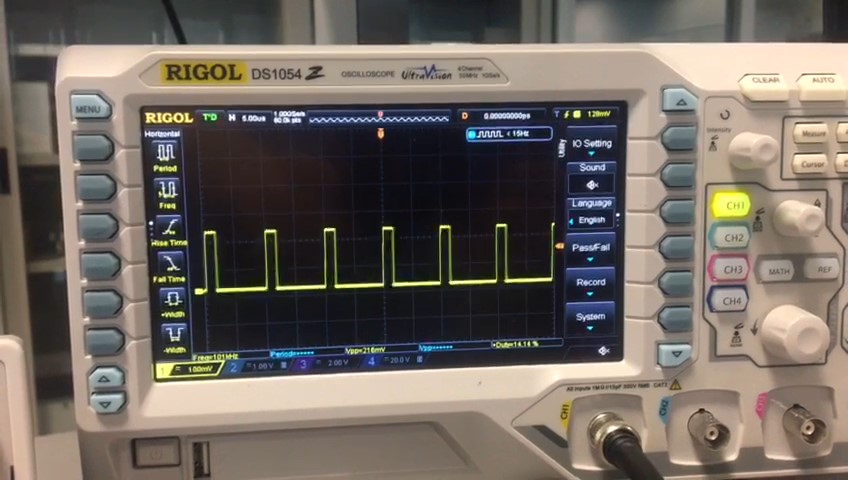
\includegraphics[scale = 0.4]{immagini/ji.jpg}
\caption{DC=25\%}
\end{figure}





\section*{2.2 LED dimmer}
The main difference of this part from the previous ones is the fact that we shift from the LL libreries to the HAL ones. After staring the PWM generation (with the HAL\_TIM\_PWM\_Start function), the duty cycle is continously incresed up to 100\% and the decreased down to 0 with the \_\_HAL\_TIM\_SET\_COMPARE function.
The given delay specifications have been satisfied exploiting the HAL function $HAL_Delay$.

If we double the period and halve the prescaler we still see a square wave at 100kHz, but the DC varies between 0 and 50\% because now the period is doubled and but we didn't double the value at witch we turn the output off.\\
Since the max DC is 50\% the led results less bright than before, but nothing else has changed.
 
 \section*{2.3 Generation of a sine waveform by means of PWM }
 
 The final task required to build a sine wave generator using the PWM function of the microcontroller. The wave is generated from 200 sample of sine used for changing the duty cycle of the PWM dynamically. In order to achieve high performances the DMA mode of the PWM is used for updating the value of the CCR register. The output signal (generated by TIM3 on the PA6 pin) needs to be filtered using an hardware low-pass filter composed of a 220$\SI{}{\ohm}$ resistance and a 1uF capacitor. 
 
\begin{figure}[h!]
	\centering
	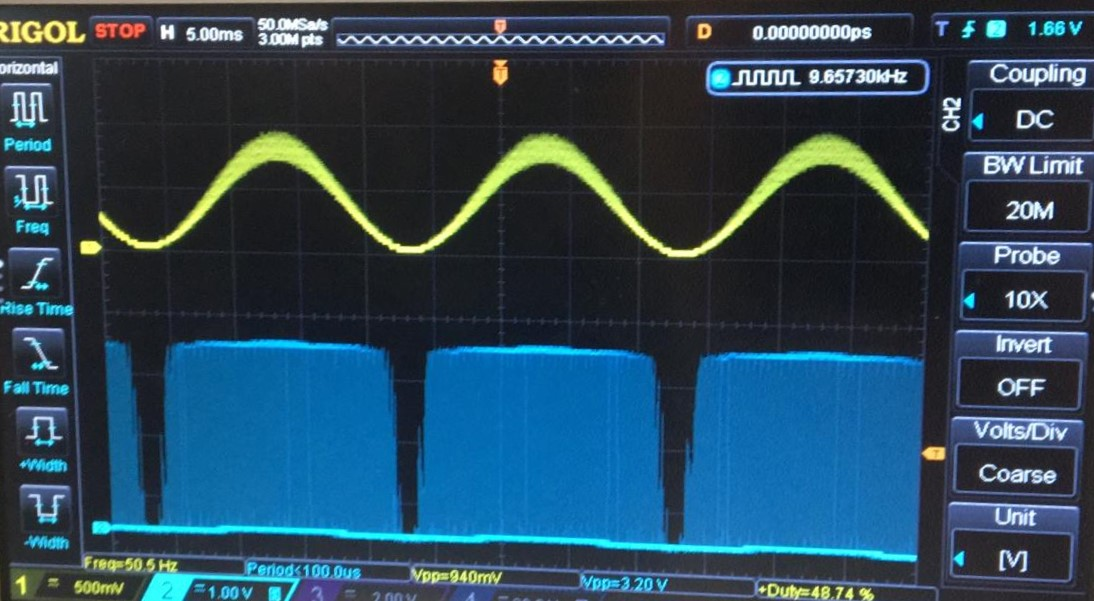
\includegraphics[scale = 0.45]{immagini/1sig.jpeg}
	\caption{Filtered sine wave and unfiltered PWM signal}
\end{figure}
\end{document}




